\scanpage{14}
\uline{Exemple}

\uline{Corollaire} Soit $G$ un préschéma en groupes de \deleted{type} \inserted{prés} finie sur $S$, \deleted{loc. noeth.} $P$ un \deleted{fibré principal} préschéma de prés. finie sur $S$ dans lequel $G$ opère, de façon que $P$ soit form. pr. hom. sous $G$. Sous ces conditions, il existe un mono de préschémas $S'\hookrightarrow S$, tel que $P\longrightarrow S$ se factorise par $P-S'$, et que \deleted{\unsure{P de} $P'$} $P$ devienne \deleted{formellement} principal hom sous $G_{S'}$ i.e. $P\longrightarrow S'$ est \deleted{plat} \uline{fid.} \uline{plat}. [De \deleted{Et} plus, $S'$ est uniquement déterminé à $S$-isom près, et est de prés. finie sur $S$].

\uline{Corollaire} Soit $u:G-H$ un hom de $S$-préschémas en groupes, \deleted{\unsure{de présentation}} $u$ de présentation finie. Supposons $\operatorname{Ker}u=N$ [qui est de prés. finie sur $S$] \uuline{plat} sur $S$. \uline{Alors} \deleted{\unsure{$u$ se factorise}} $G/N$ \uline{existe}.
\figure{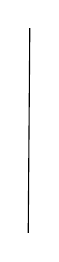
\begin{tikzpicture}[x=1cm,y=1cm]\draw (0,0)--(.02,2.6);\end{tikzpicture}}
\mspage{13}
